% Very simple template for lab reports. Most common packages are already included.
\documentclass[a4paper, 11pt]{article}
\usepackage[utf8]{inputenc} % Change according your file encoding
\usepackage{graphicx}
\usepackage{url}

%opening
\title{Report 2: Rudy homework report}
\author{Douglas Hammarstam}
\date{\today{}}

\begin{document}

\maketitle

\section{Introduction}

\textit{In this project, a simple web server has been implemented.}

In this seminar, the main topic covered was the HTTP-protocol and how to parse it using Erlang.
Furthermore, the seminar covered how to use the gen-tcp
package in order to receive network HTTP-requests and handle the requests by
using above mentioned parsing of the HTTP request.  

This is important in order to get an understanding of how to use Erlang in order to efficiently parse HTTP-requests (strings)
using recursion.

It is also important in order to understand basic Erlang features like recursion, pattern-matching aswell as spawning processes in order to distribute an application on multiple threads.

\section{Main problems and solutions}

\textit{

The first problem in the assignment was to parse the incoming HTTP-request. This was done by dividing the problem into different sections;
Firstly, parsing the method used in the request (GET). Then the URL is received by parsing each character after the space (32) character after the GET string until we reach another space character (32).
Secondly, we get the HTTP-version (v10 or v11) by simply pattern matching the string to either of those values.
Thirdly, we parse a line-break character followed by the headers, which we also recursively parse each 


Summarize your problems, proposed solutions, etc. You do not
  need to copy\&paste your code. Only if needed, you may write down
  small code snipeds to show how you have solved a specific
  problem/question.}


Did you find any specific problem with the development of your
solution?  How did you solve it?

If you want to give a code example you can do it uing the verbatim environment.
\begin{verbatim}
this(X) ->
    Y = is(X),
    a(test(Y)).
\end{verbatim}

\section{Evaluation}

\textit{If needed, you may provide figures or tables with main results
  evaluating your proposals. For each seminar, we will provide you
  with some guidance on which kind of evaluation you should do.}


And Figures \ref{fig:results1} and \ref{fig:results2 } shows how to
add a figure with some results. These figures have been created with
gnuplot. There are tons of different kinds of plots that can be
generated with gnuplot. Make sure to check out
\url{http://gnuplot.info/demo/} and look at them so you can see what
can you do with this program.


\begin{figure}
  \begin{center}
    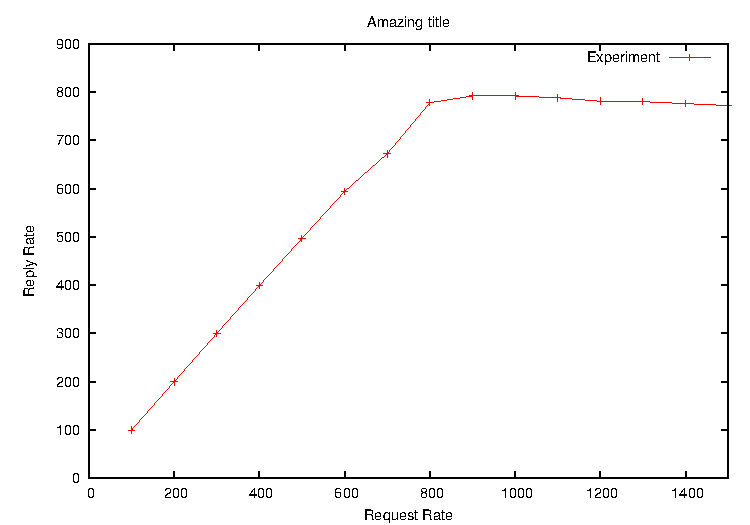
\includegraphics{results1.pdf}
    \caption{Some random results 1}
    \label{fig:results1}
  \end{center}
\end{figure}


\begin{figure}
  \begin{center}
    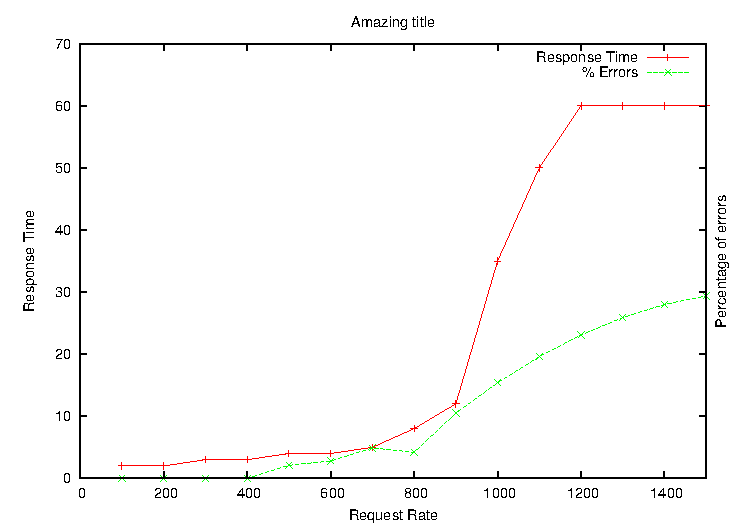
\includegraphics{results2.pdf}
    \caption{Some random results 2}
    \label{fig:results2}
  \end{center}
\end{figure}

To obtain these figures you have to:
\begin{enumerate}

\item Create the data file from the experiments (look at file
  experiment.dat)

\item Create a gnuplot file to create a figure in eps format (look at
  files results1.plot and results2.plot). These files may be very
  complex. But for the results we want to show, these examples are
  enough. To create the eps figures, execute in terminal:

\begin{verbatim}
$> gnuplot results1.plot 
\end{verbatim}

\item As pdflatex does not recognize eps files, you must convert them
  to pdf files. This is done by (it will generate a file
  results1.pdf):

\begin{verbatim}
$> epstopdf results1.eps
\end{verbatim}

\item That's it! Just include the figure as shown in this template and
  compile the latex as explained in the document ``Introduction to
  \LaTeXe''.

\end{enumerate}


If you want, you can also create a table of results as Table
\ref{tab:results}. If you look at the template code, you will see how
to do a table in \LaTeX.

\begin{table}[h]
\centering
\begin{tabular}{lcc}
First column & Second column & Third column\\\hline
Case 1 & 1.1 & 1.2\\\hline
Case 2 & 2.1 & 2.2\\\hline
Case 3 & 3.1 & 3.2\\\hline
\end{tabular}
\caption{Some random results in a table}
\label{tab:results}
\end{table}

\section{Conclusions}

\textit{Change the layout of this template as you want. It's only for
  your guidance but if you feel that you need a different structure,
  feel free to change it. The report should not be too long ($\approx$
  2-3 pages).}

What have you learnt from the problem presented?
Was it useful?


\end{document}
